\documentclass[12pt]{article}

\usepackage{sbc-template}
\usepackage{graphicx,url}
\usepackage[utf8]{inputenc}
\usepackage{subfigure}
\usepackage[english]{babel}
\usepackage{wasysym}
\usepackage[ruled,vlined]{algorithm2e}
\usepackage{fancyvrb}
\usepackage{float}
\usepackage{tikz}

% para quebrar urls de forma adequada
\def\UrlBigBreaks{\do\/\do-\do:}



\usetikzlibrary{positioning, calc, decorations.pathreplacing, arrows.meta}
\sloppy

\renewcommand{\email}[1]{\\\mbox{}\\[-6pt]\footnotesize\ttfamily\begin{tabular}[t]{@{}c@{}}#1\end{tabular}}

\newcommand{\placeholderfigure}[3]{%
\begin{figure}[htb]
\centering
\fbox{%
\begin{minipage}[c][#1][c]{0.9\linewidth}
\centering
\textbf{#2}
\end{minipage}}
\caption{#3}
\end{figure}
}


\title{\$1 Yacht Sale: Tampering with Signed PDFs in Plain Sight}

\author{Enzo R. Brum\inst{1}, Frederico Schardong\inst{1}, Ricardo Custódio\inst{1}}


\address{Laboratório de Segurança em Computação (LabSEC) -- Departamento\\
de Informática e Estatística (INE) -- Universidade Federal\\
de Santa Catarina -- Brazil
\email{enzo.brum@grad.ufsc.br\\
frederico.schardong@ufsc.br\\
ricardo.custodio@ufsc.br}
}

\begin{document}

\maketitle

\begin{abstract}
	The Portable Document Format (PDF) is a popular way of sharing electronic documents. It is a format used across fields to represent official documents, many of which require strong guarantees that no unauthorized modifications are made to their contents. Digital signatures can be used to protect both the integrity and authenticity of a document, allowing an entity, whether a person, business, or service, to testify to one specific state of the document such that any non-permitted modification, for example altering the value of a contract or a health prescription, invalidates the signature. In this paper we introduce two novel attack classes that abuse flaws in the PDF specification to visually modify a page of a signed document without invalidating the signature or warning the user: Appearance Substitution Attack (ASA) and Signature Field Duplication Attack (SFDA). While previous works already explored incremental updates, we tap into modifications to the signature field itself, a specific kind of update that has yet to be fully explored. Our evaluation found that 12 out of 15 tested GUI applications and 2 popular verification libraries were at least partially vulnerable to one of the attack classes. We also propose countermeasures and specification improvements for fixing both.


\end{abstract}


\section{Introduction}

The Portable Document Format (PDF) allows documents to be represented consistently across devices and is the de facto standard for electronic documents, common in countless workflows around the globe. Between 2025 and 2026, more than 320 billion documents were opened and more than 8 billion were signed using Adobe Reader~\cite{adobe-sign-2026}. PDFs are used to represent contracts, invoices, agreements, and many other kinds of official documents. The format is specified by ISO~32000-2~\cite{iso32000-2} and implemented by a wide range of programs~\cite{adobereader,foxitreader,libreoffice}.

To ensure that the state of a PDF document is trustworthy, the standard defines PDF signatures, which use asymmetric cryptography over the signed bytes of the document to attest that a given state was approved by the signer and to protect it from subsequent modifications. Their use is legally recognized in Brazil by Law~14.063~\cite{lei14063}, in the European Union by the eIDAS Regulation~\cite{eidas2014}, and in the United States by the Electronic Signatures in Global and National Commerce Act (ESIGN)~\cite{esign2000}, each granting signed digital documents evidentiary weight comparable to handwritten ones.

PDF signatures, however, are not unbreakable~\cite{one-trillion-dollar-refund,shadow-attacks,pdf-certification-attack}. In this paper we present two attacks that visually alter a page of a signed document without invalidating the signature or triggering modification warnings from verifiers: the Appearance Substitution Attack (ASA) and the Signature Field Duplication Attack (SFDA). As shown in Figure~\ref{fig:attack-example}, an attacker can change the value of a signed contract while the verifier continues to report the signature as valid. The only requirement is access to the signed document.

As in prior work, we target \texttt{incremental updates}. Existing attacks have either abused verifier flaws to hide changes introduced through such updates~\cite{one-trillion-dollar-refund}, required attacker access to the document before signing~\cite{shadow-attacks}, or exploited specific permission levels of modification-control mechanisms~\cite{pdf-certification-attack}. Both ASA and SFDA, instead, target the \texttt{signature field} itself. While ASA directly modifies an existing signature field, the SFDA duplicates one while placing attacker-controlled visual content on any page of the document. Although prior work~\cite{pdf-certification-attack} flagged the combination of \texttt{incremental updates} and signature fields as dangerous, the potential of that combination had not been fully explored.

The contributions of this paper are three fold: (i) we tested 15 GUI applications and 2 popular programming libraries, finding 14 of the 17 to be at least partially vulnerable to of the two attacks; (ii) we propose countermeasures at the specification, verifier, and tooling levels; and (iii) release an open-source tool that detects both attacks in a given PDF.
%
The remainder of this paper is organized as follows. Section~\ref{sec:background} introduces the PDF concepts relevant to the attacks, while Section~\ref{sec:threat-model} defines the threat model. Then, Section~\ref{sec:attack-definitions} presents ASA and SFDA in detail, Section~\ref{sec:methodology} describes the testing methodology, and Section~\ref{sec:evaluation} reports our evaluation. Next, Section~\ref{sec:countermeasures} discusses countermeasures, while Section~\ref{sec:related-works} relates the attacks to prior work, Section~\ref{sec:ethics} details our ethical considerations and disclosure process, and finally Section~\ref{sec:conclusion} concludes the paper.


\begin{figure}[htb]
	\centering
	\subfigure[Original signed contract.]{\includegraphics[width=0.47\linewidth]{fig_contract_original.png}}
	\hfill
	\subfigure[After attack.]{\includegraphics[width=0.463\linewidth]{fig_contract_after_attack.png}}
	\caption{\label{fig:attack-example} Example of a contract in which the contracted value has been altered after signing, while the signature is still reported as valid.}
\end{figure}


\section{Background} \label{sec:background}

% TODO: may need to make it smaller if lacking space later on. good enough for now.

\subsection{PDF Structure and Incremental Updates}

A PDF document consists of four parts: (i) a header declaring the PDF version; (ii) a body containing the document's objects; (iii) a cross-reference (xref) table mapping each object to its byte offset; and (iv) a trailer pointing to both the xref table and the document's root object.
%
An object is a number, a string, a name, an array, a dictionary, or a stream. In the body, each object appears either as a \emph{direct value}, written inline at the point of use, or as an \emph{indirect object}, declared with a unique identifier of the form \texttt{N M obj} and referenced from other objects by \texttt{N M R}. In Figure~\ref{fig:pdf-structure}(a), the \texttt{Catalog}, a dictionary, is declared as \texttt{1 0 obj} and references a \texttt{Pages} dictionary (\texttt{2 0 R}), which links to the individual pages of the document, and an \texttt{AcroForm} dictionary (\texttt{3 0 R}), which describes any interactive form fields that users can fill or modify. The \texttt{Catalog} is the entry point of the document, and every other indirect object is reached by following references from it.


%\begin{noindent}
\begin{figure}[htb]
	\centering
	\begin{minipage}[b]{0.44\linewidth}
		\centering
		\begin{Verbatim}[frame=single,fontsize=\scriptsize]
1 0 obj  % Catalog
<< /Type /Catalog
   /Pages    2 0 R
   /AcroForm 3 0 R >>
endobj

2 0 obj  % Pages
<< /Kids [4 0 R]
   /Count 1 >>
endobj

3 0 obj  % AcroForm
<< /Fields [6 0 R] >>
endobj

4 0 obj  % Page
<< /Parent 2 0 R
   /Annots [6 0 R] >>
endobj
		\end{Verbatim}

		{\footnotesize (a) Skeleton object tree.}
	\end{minipage}%
	\hfill
	\begin{minipage}[b]{0.50\linewidth}
		\centering
		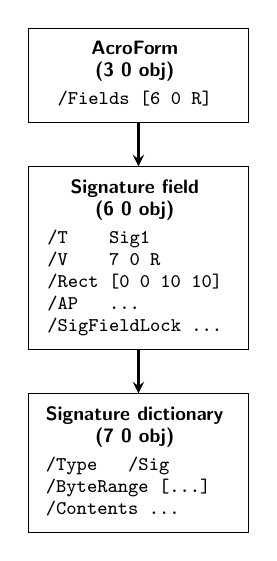
\begin{tikzpicture}[
			font=\scriptsize,
			dict/.style={draw, rectangle, align=left, inner sep=4pt, minimum width=2.8cm},
			arr/.style={->, thick, >=stealth},
		]
			\node[dict] (acro) {%
				\begin{tabular}{@{}l@{}}
					\multicolumn{1}{@{}c@{}}{\textbf{\sffamily AcroForm}}\\
					\multicolumn{1}{@{}c@{}}{\scriptsize\textbf{\sffamily (3 0 obj)}}\\[2pt]
					\texttt{\textbf{/Fields [6 0 R]}}
				\end{tabular}
			};
			\node[dict, below=0.55cm of acro] (field) {%
				\begin{tabular}{@{}l@{}}
					\multicolumn{1}{@{}c@{}}{\textbf{\sffamily Signature field}}\\
					\multicolumn{1}{@{}c@{}}{\scriptsize\textbf{\sffamily (6 0 obj)}}\\[2pt]
					\texttt{/T \ \ \ Sig1}\\
					\texttt{\textbf{/V \ \ \ 7 0 R}}\\
					\texttt{/Rect [0 0 10 10]}\\
					\texttt{/AP \ \ ...}\\
					\texttt{/SigFieldLock ...}
				\end{tabular}
			};
			\node[dict, below=0.55cm of field] (sigdict) {%
				\begin{tabular}{@{}l@{}}
					\multicolumn{1}{@{}c@{}}{\textbf{\sffamily Signature dictionary}}\\
					\multicolumn{1}{@{}c@{}}{\scriptsize\textbf{\sffamily (7 0 obj)}}\\[2pt]
					\texttt{/Type \ \ /Sig}\\
					\texttt{/ByteRange [...]}\\
					\texttt{/Contents ...}
				\end{tabular}
			};
			\draw[arr] (acro.south)  -- (field.north);
			\draw[arr] (field.south) -- (sigdict.north);
		\end{tikzpicture}

		{\footnotesize (b) Signature field (object 6) and its signature dictionary.}
	\end{minipage}
	\caption{PDF object structure. (a) A skeleton object tree: the \texttt{Catalog} references the \texttt{Pages} and \texttt{AcroForm} dictionaries, and the signature field (object~6) is reached from both the \texttt{AcroForm}'s \texttt{/Fields} and its page's \texttt{/Annots}. (b) That signature field and the \texttt{signature dictionary} it references through \texttt{/V}.\label{fig:pdf-structure}}
\end{figure}
%\end{noindent}


% \subsection{Incremental Updates}

When handling updates, a PDF processor can append changes to the end of the file rather than
overwriting existing content. Modified objects are appended after the \texttt{\%EOF} marker, and a new \texttt{xref} table and \texttt{trailer} are added, creating a new \texttt{revision} of the document.
%
Most PDF readers merge all \texttt{revisions} into a unified view, though some (such as Adobe Acrobat Reader~\cite{adobereader}) also expose tools for inspecting each revision individually.


%\begin{noindent}
%\begin{figure}[htb]
   % \centering
   % \begin{tikzpicture}[
   %     box/.style={draw, minimum width=3cm, minimum height=0.6cm, align=center, font=\small},
   %     orig/.style={box, fill=blue!10},
   %     new/.style={box, fill=orange!30},
   % ]
   %     % original revision (left column)
   %     \node[orig]                  (h1) {Header};
   %     \node[orig, below=0pt of h1] (b1) {Body};
   %     \node[orig, below=0pt of b1] (x1) {xref table};
   %     \node[orig, below=0pt of x1] (t1) {Trailer};
   %     \node[above=4pt of h1, font=\small\bfseries] {Revision 1};
%
%        % updated revision (right column)
%        \node[orig, right=5cm of h1] (h2) {Header};
%        \node[orig, below=0pt of h2]   (b2) {Body};
%        \node[orig, below=0pt of b2]   (x2) {xref table};
%        \node[orig, below=0pt of x2]   (t2) {Trailer};
%        \node[new,  below=0pt of t2]   (bu) {Updated body};
%        \node[new,  below=0pt of bu]   (xu) {New xref table};
%        \node[new,  below=0pt of xu]   (tu) {New trailer};
%        \node[above=4pt of h2, font=\small\bfseries] {Revision 2};
%
%        % arrow between columns, label above
%        \coordinate (la) at ($(h1.east)!0.5!(t1.east)$);
%        \draw[-{Stealth[length=3mm]}, thick, dashed] ($(la)+(0.25,0)$)
%            -- node[sloped, above, font=\small\itshape] {incremental update}
%            ($(xu.west)+(-0.25,0)$);
%    \end{tikzpicture}
%    \caption{Incremental update: the updated objects, a new xref table, and a new trailer are appended after the original revision.\label{fig:incremental-update}}
%\end{figure}
%\end{noindent}


\subsection{Signature Field} \label{sec:sig-field}

A \texttt{signature field} is a specialized form field that acts as a container for a PDF digital signature. Each \texttt{signature field} is registered in the document's \texttt{AcroForm} dictionary via the \texttt{/Fields} entry and is associated with a single page. Its most relevant attributes are (i) \texttt{/T}, a name uniquely identifying the field within the document; (ii) \texttt{/V}, the reference to the \texttt{signature dictionary} that defines the digital signature itself; (iii) \texttt{/AP}, which defines the field's visual appearance; (iv) \texttt{/Rect}, which specifies the field's position and dimensions on the page; and (v) \texttt{/SigFieldLock}, which controls field-level modification permissions (Section~\ref{sec:doc-mod-perm}). Figure~\ref{fig:pdf-structure}(b) illustrates this structure.

The PDF specification calls \emph{filling} the operation that supplies input to a form field. For a signature field, filling means updating at least the \texttt{/V} entry by attaching a new \texttt{signature dictionary}, but it can also mean more.



% \subsection{Digital Signatures}

A document is digitally signed by appending a new \texttt{signature field}, linked to a page and to a new \texttt{signature dictionary}, as an \texttt{incremental update}. Each \texttt{signature dictionary} contains the user's certificate and a byte range covering the full document as it existed at signing time; the digital signature is computed over that byte range using the user's private key and stored within the \texttt{signature dictionary}.

As shown in Figure~\ref{fig:multiple-signatures}, appending signatures as incremental updates naturally supports multiple signatures on the same document. A new signature can be appended without invalidating any prior one, since the bytes covered by earlier signatures remain unchanged.

%\begin{noindent}
\begin{figure}[htb]
    \centering
    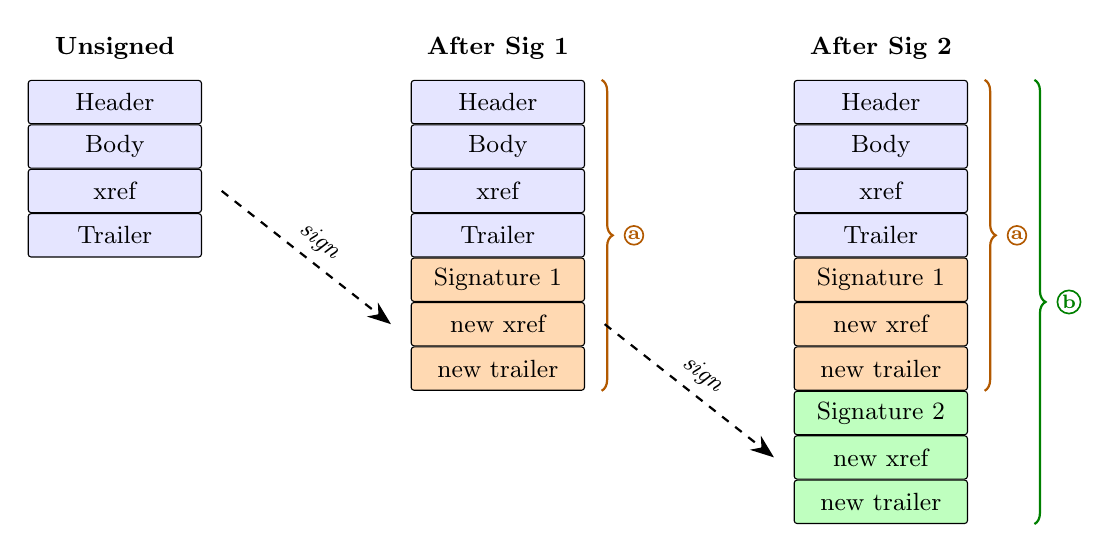
\begin{tikzpicture}[
        >={Stealth[length=2mm, width=1.6mm]},
        box/.style={draw, line width=0.4pt, rounded corners=1pt,
                    minimum width=2.2cm, minimum height=0.55cm, align=center, font=\small},
        orig/.style={box, fill=blue!10},
        sig1/.style={box, fill=orange!30},
        sig2/.style={box, fill=green!25},
        brc1/.style={decorate, decoration={brace, amplitude=4pt, raise=2pt, mirror},
                     thick, draw=orange!70!black},
        brc2/.style={decorate, decoration={brace, amplitude=4pt, raise=2pt, mirror},
                     thick, draw=green!50!black},
        brlbl1/.style={font=\footnotesize, text=orange!70!black},
        brlbl2/.style={font=\footnotesize, text=green!50!black},
        mark1/.style={circle, draw=orange!70!black, fill=white, line width=0.6pt,
                      inner sep=0.5pt, font=\scriptsize\bfseries, text=orange!70!black},
        mark2/.style={circle, draw=green!50!black,  fill=white, line width=0.6pt,
                      inner sep=0.5pt, font=\scriptsize\bfseries, text=green!50!black},
    ]
        % col 1: unsigned document
        \node[orig]                  (Uh) {Header};
        \node[orig, below=0pt of Uh] (Ub) {Body};
        \node[orig, below=0pt of Ub] (Ux) {xref};
        \node[orig, below=0pt of Ux] (Ut) {Trailer};
        \node[above=4pt of Uh, font=\small\bfseries] {Unsigned};

        % col 2: state after signing with Sig 1
        \node[orig, right=2.65cm of Uh]    (Ah)  {Header};
        \node[orig, below=0pt of Ah]    (Ab)  {Body};
        \node[orig, below=0pt of Ab]    (Ax)  {xref};
        \node[orig, below=0pt of Ax]    (At)  {Trailer};
        \node[sig1, below=0pt of At]    (As)  {Signature 1};
        \node[sig1, below=0pt of As]    (Axn) {new xref};
        \node[sig1, below=0pt of Axn]   (Atn) {new trailer};
        \node[above=4pt of Ah, font=\small\bfseries] {After Sig 1};

        % col 3: state after signing with Sig 2
        \node[orig, right=2.65cm of Ah]    (Bh)   {Header};
        \node[orig, below=0pt of Bh]    (Bb)   {Body};
        \node[orig, below=0pt of Bb]    (Bx)   {xref};
        \node[orig, below=0pt of Bx]    (Bt)   {Trailer};
        \node[sig1, below=0pt of Bt]    (Bs1)  {Signature 1};
        \node[sig1, below=0pt of Bs1]   (Bxn1) {new xref};
        \node[sig1, below=0pt of Bxn1]  (Btn1) {new trailer};
        \node[sig2, below=0pt of Btn1]  (Bs2)  {Signature 2};
        \node[sig2, below=0pt of Bs2]   (Bxn2) {new xref};
        \node[sig2, below=0pt of Bxn2]  (Btn2) {new trailer};
        \node[above=4pt of Bh, font=\small\bfseries] {After Sig 2};

        % brace marker position along brace (0 = bottom, 1 = top); tune to taste
        \def\sigrangepos{0.5}

        % col 2 brace: Sig 1 byte range
        \draw[brc1] ([xshift=4pt]Atn.south east) -- ([xshift=4pt]Ah.north east)
            node[pos=\sigrangepos, right=10pt, mark1] {a};

        % col 3 braces: inner Sig 1, outer Sig 2
        \draw[brc1] ([xshift=4pt]Btn1.south east)  -- ([xshift=4pt]Bh.north east)
            node[pos=\sigrangepos, right=10pt, mark1] {a};
        \draw[brc2] ([xshift=22pt]Btn2.south east) -- ([xshift=22pt]Bh.north east)
            node[pos=\sigrangepos, right=10pt, mark2] {b};

        % incremental update arrows: col 1 -> new xref of Sig 1; col 2 (xref of Sig 1) -> new xref of Sig 2
        \coordinate (la1) at ($(Uh.east)!0.5!(Ut.east)$);
        \draw[-{Stealth[length=3mm]}, thick, dashed] ($(Ux.east)+(0.25,0)$)
            -- node[sloped, above, font=\small\itshape] {sign}
            ($(Axn.west)+(-0.25,0)$);

        \draw[-{Stealth[length=3mm]}, thick, dashed] ($(Axn.east)+(0.25,0)$)
            -- node[sloped, above, font=\small\itshape] {sign}
            ($(Bxn2.west)+(-0.25,0)$);
    \end{tikzpicture}

    \vspace{2pt}
    {\footnotesize
    \tikz[baseline=-0.6ex]\node[circle, draw=orange!70!black, fill=white, line width=0.6pt,
        inner sep=0.5pt, font=\scriptsize\bfseries, text=orange!70!black] {a};~content protected by first signature\quad
    \tikz[baseline=-0.6ex]\node[circle, draw=green!50!black, fill=white, line width=0.6pt,
        inner sep=0.5pt, font=\scriptsize\bfseries, text=green!50!black] {b};~content protected by second signature}

    \caption{Each signing applies an incremental update; the new signature covers all bytes that existed at signing time, so earlier signatures remain valid.\label{fig:multiple-signatures}}
\end{figure}
%\end{noindent}



\subsection{Modification Permission Mechanism} \label{sec:doc-mod-perm}

Because \texttt{incremental updates} preserve all prior bytes, visual content can be modified after signing without technically invalidating the signature. An attacker could, for example, alter a page or inject an annotation via an incremental update while leaving the signed byte range intact, all within the boundaries of the specification~\cite{iso32000-2}. In response, most verifiers~\cite{adobereader,foxitreader,libreoffice} either treat such post-signing modifications as invalidating the signature or surface a warning to the user.

The specification also provides mechanisms that make signatures sensitive to specific classes of modifications. \texttt{DocMDP} defines which types of modification are permitted before the signature is considered broken; \texttt{FieldMDP} locks specific form fields so that any change to them invalidates the signature; and \texttt{SigFieldLock} can do both capabilities. \texttt{DocMDP} and \texttt{FieldMDP} reside in the signature dictionary, while \texttt{SigFieldLock} is referenced by the signature field itself and its value is copied into \texttt{FieldMDP} at signing time. \texttt{DocMDP} and \texttt{SigFieldLock} share three permission levels: (i) level 1 forbids any modification; (ii) level 2 permits form fill-in and additional signatures; and (iii) level 3 additionally permits annotation creation, modification, and deletion.

As described in~\cite{pdf-certification-attack}, PDF distinguishes between \emph{approval} signatures, which attest to the document's state, and a \emph{certification} signature, which additionally governs which modifications are permissible. A document may carry at most one certification signature, which must appear first; any number of approval signatures may follow. \texttt{DocMDP} is exclusive to certification signatures. \texttt{FieldMDP} and \texttt{SigFieldLock} may be used by either kind. Since PDF 2.0~\cite{iso32000-2}, \texttt{SigFieldLock} carries the same expressive power as \texttt{DocMDP}, allowing approval signatures to impose document-level modification restrictions as well. %Table~\ref{tab:mdp-mechanisms} summarizes the differences.

%\begin{table}[htb]
%	\centering
%	\small
%	\begin{tabular}{@{}l p{4.8cm} l@{}}
%		\hline
%		\textbf{Mechanism}    & \textbf{Scope}                                          & \textbf{Allowed in}           \\
%		\hline
%		\texttt{DocMDP}       & whole document, per permission level                    & certification signatures only \\
%		\texttt{FieldMDP}     & listed form fields only                                 & any signature                 \\
%		\texttt{SigFieldLock} & listed form fields, plus whole document (since PDF~2.0) & any signature                 \\
%		\hline
%	\end{tabular}
%	\caption{Capabilities of each PDF modification-permission mechanism.\label{tab:mdp-mechanisms}}
%\end{table}


\section{Threat Model} \label{sec:threat-model}

Our threat model follows the method introduced by~\cite{one-trillion-dollar-refund}. The attacker's goal is to alter the visual content of a signed PDF while ensuring that signature verifiers continue to report the original signature as valid and raise no warning about post-signing modifications. We assume the attacker has obtained a PDF carrying a digital signature that the target verifier already trusts and considers valid.

The \emph{victim} is the person, organization, or service that needs to establish whether a document carries a trusted signature. The \emph{signer} is the party that originally signed the document and, in doing so, configured any modification-permission mechanisms.

We consider two classes of verifier: Graphical User Interface (GUI) applications and programming libraries. The distinction matters because each class exposes a different surface to the user, and our attacks succeed in different ways on each.

\subsection{User Interface Verifiers}

GUI verifiers show signature verification results through multiple visual components, such as a top-bar banner and a details panel. We reuse the UI layer abstraction of~\cite{one-trillion-dollar-refund} to refer to these components, and restate below the two layers relevant to our attacks.

\textbf{UI-Layer 1} is the top-bar validation status. Most GUI verifiers display this banner immediately upon opening the document and use it to summarize whether all signatures in the document are valid. Owing to its prominence, it is typically the first cue a user inspects when assessing the document's authenticity.

\textbf{UI-Layer 2} carries detailed per-signature information, such as the signer's name and certificate chain. It is generally not opened automatically, the user must open a dedicated panel before this information becomes visible.

\subsection{Programming Libraries}

Programming libraries expose a binary verdict and a detailed report describing every check performed for each verified signature. We collapse both into a single abstraction, the \textbf{API-Layer}, since they are returned together in the same function response and any developer consuming the library has access to both at once.

In this abstraction, the API-Layer answers two questions: whether the signature is considered valid, and whether any warning should be noted alongside the verdict. For instance, one of such warnings can be that the verifier detected an uncommon or post-signing modification but still accepts the signature as valid.

\subsection{Winning Conditions} \label{sec:winning-conditions}

For each UI layer for GUI verifiers or the single API-Layer for library verifiers, we classify the outcome of an attack as follows~\cite{one-trillion-dollar-refund}. The output is \emph{vulnerable} (\CIRCLE) when it reports the signature as valid without flagging a post-signing modification. It is \emph{partially vulnerable} (\LEFTcircle) when it reports the signature as valid but raises a warning that the document was modified. It is \emph{secure} (\Circle) when it flags the signature as invalid.

For GUI verifiers, an attack is \emph{successful} when both UI layers are vulnerable, and \emph{partially successful} when UI-Layer~1 is vulnerable while UI-Layer~2 is either \emph{partially vulnerable} or \emph{secure}. We treat partial success as meaningful because an inattentive user may rely solely on the top-bar banner and overlook the warning surfaced in the detail panel, accepting a modified document despite the recorded discrepancy. For library verifiers, an attack is \emph{successful} when the API-Layer is vulnerable, and \emph{partially successful} when it is partially vulnerable; the same reasoning applies, since a developer may consume only the binary verdict and ignore the accompanying warnings.


\section{Breaking Digital Signature Verifiers} \label{sec:attack-definitions}

Our attacks exploit two underspecified aspects of the PDF specification~\cite{iso32000-2}. By modifying a signature field's existing entries, an attacker can place arbitrary visual content on a page, as in Figure~\ref{fig:attack-example}, without invalidating the signature in affected verifiers.

\subsection{Appearance Substitution Attack (ASA)}

% 1. reexplain /Rect and /AP
% 2. explain that /Rect can be resized and /AP can be overwritten as to change what's actualy shown on page. -> point to figure with an already signed document with a common stamp -> change it so rect compasses whole page, the stamp is kept and text is changed. show virtual square outline so people see it
% 3. argument the spec is flawed, provide exact wording and say it does NOT necessarily restrict such attack.

As described in Section~\ref{sec:sig-field}, a signature field's \texttt{/Rect} entry defines the region of the page occupied by the field, while its \texttt{/AP} entry defines the appearance drawn inside that region. For signatures with a visible component, \texttt{/Rect} typically identifies a small area of the page containing the signer's name or stamp, and \texttt{/AP} stores the corresponding visual representation. For signatures without a visible component, \texttt{/Rect} commonly contains a zero-area rectangle, and \texttt{/AP} is absent.

The \texttt{/Rect} and \texttt{/AP} entries can be abused to turn a signature field into a vehicle for arbitrary visual content. Expanding \texttt{/Rect} to cover a larger region, or even the entire page, increases the area in which the field appearance can be rendered. Replacing \texttt{/AP} then changes what is drawn. As shown in Figure~\ref{fig:rect-ap-abuse}, an attacker can start from a document that already contains a visible signature, preserve the original signature appearance, and add a small malicious modification elsewhere on the page by carefully crafting the replacement appearance stream. When the existing signature is invisible, the same outcome is achieved by creating a new \texttt{/AP} and enlarging \texttt{/Rect} from its default value.

As discussed in Section~\ref{sec:doc-mod-perm}, permission levels two and three of \texttt{DocMDP} and \texttt{SigFieldLock} allow form fields to be filled through an incremental update without invalidating the protected signature. Since a signature field is itself a form field, the specification does not explicitly rule out filling such a field after a prior signature has been applied. In fact, the relevant ISO wording leaves room for interpretation on what ``filling'' means:

\begin{quote}
	\emph{[Filling in (signing) the signature field entails updating at least the \texttt{/V} entry and usually also the \texttt{/AP} entry of the associated widget annotation. (Section 12.7.5.5 of ISO~32000-2~\cite{iso32000-2})]}
\end{quote}

The phrase ``at least'' suggests that filling a signature field is not necessarily limited to updating \texttt{/V} and \texttt{/AP}. Under a permissive interpretation, other field entries, including \texttt{/Rect}, could also be treated as part of the same filling operation. This ambiguity enables ASA to be applied to documents protected by modification-permission mechanisms while remaining within the class of changes that affected verifiers accept as non-invalidating.

\begin{figure}[htb]
	\centering
	% (a) visual outcome
	\begin{minipage}{\linewidth}
		\centering
		\begin{tikzpicture}[
				img/.style={inner sep=0pt, outer sep=0pt},
				lbl/.style={font=\small\itshape, yshift=-2pt},
			]
			\node[img] (og)  {\includegraphics[width=0.44\linewidth]{og_outlined_stamp_rect.png}};
			\node[img, right=0.6cm of og] (mod) {\includegraphics[width=0.44\linewidth]{mod_outlined.png}};
			\node[lbl, below=2pt of og]  {original signed contract};
			\node[lbl, below=2pt of mod] {after ASA};
			\draw[->, very thick, >={Stealth[length=3mm, width=2mm]}]
			(og.east) -- (mod.west);
		\end{tikzpicture}\\[3pt]
		{\footnotesize (a) Visual outcome. Cyan outlines mark the signature field's \texttt{/Rect}: a small region around the original stamp on the left, expanded to cover the whole page on the right. Red outlines on the right highlight the original stamp redrawn at its original location and the malicious value that overwrites \texttt{\$\,1,000,000,000.00} with \texttt{\$\,1}.}
	\end{minipage}\\[12pt]
	% (b) structural view
	\begin{minipage}{\linewidth}
		\centering
		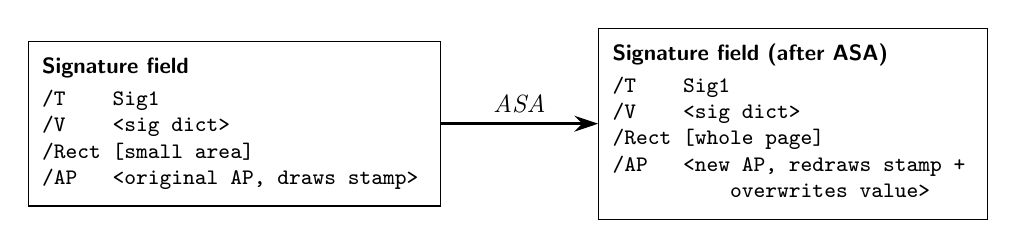
\begin{tikzpicture}[
				dict/.style={draw, rectangle, align=left, inner sep=5pt, font=\footnotesize},
				note/.style={font=\small\itshape},
			]
			% original field
			\node[dict] (ogfield) {%
				\begin{tabular}{@{}l@{}}
					\textbf{\sffamily Signature field} \\[2pt]
					\texttt{/T \ \ \ Sig1}             \\
					\texttt{/V \ \ \ <sig dict>}       \\
					\texttt{/Rect [small area]}        \\
					\texttt{/AP \ \ <original AP, draws stamp>}
				\end{tabular}
			};

			% modified field
			\node[dict, right=2.0cm of ogfield] (modfield) {%
				\begin{tabular}{@{}l@{}}
					\textbf{\sffamily Signature field (after ASA)} \\[2pt]
					\texttt{/T \ \ \ Sig1}                         \\
					\texttt{/V \ \ \ <sig dict>}                   \\
					\texttt{/Rect [whole page]}                    \\
					\texttt{/AP \ \ <new AP, redraws stamp +}      \\
					\hspace*{5em}\texttt{overwrites value>}
				\end{tabular}
			};

			\draw[->, very thick, >={Stealth[length=3mm, width=2mm]}]
			(ogfield.east) -- node[above, note] {ASA} (modfield.west);
		\end{tikzpicture}\\[3pt]
		{\footnotesize (b) Abstract structural change. \texttt{/T} and \texttt{/V} are preserved, while \texttt{/Rect} is enlarged to span the whole page and a new \texttt{/AP} is created that redraws the original stamp at its original location and overwrites the contracted value elsewhere on the page.}
	\end{minipage}
	\caption{ASA applied to a contract signed at gov.br: (a) visual example of the attack; (b) abstract structural view of the modified signature field.\label{fig:rect-ap-abuse}}
\end{figure}


\subsection{Signature Field Duplication Attack (SFDA)}

A related attack exists when instead of mutating an existing signature field, the attacker introduces a \emph{new} signature field through an incremental update and sets its \texttt{/V} entry to point at the signature dictionary of a signature already present in the document. The duplicated field is registered in the \texttt{AcroForm} dictionary alongside the original and can be placed on any page, with attacker-controlled \texttt{/Rect} and \texttt{/AP} entries. Because the bytes covered by the original signature are untouched, the cryptographic verification of that signature continues to succeed, and affected verifiers render the duplicated field as a second valid signature. An example of the resulting document is shown in Figure~\ref{fig:sfda-example}.

SFDA is closely related to the Sneaky Signature Attack of~\cite{pdf-certification-attack} but differs in one fundamental respect: it does not require the attacker to produce a fresh signature trusted by the verifier. Whereas the Sneaky Signature Attack appends an attacker-controlled signature dictionary, SFDA reuses the legitimate one. This makes the attack particularly damaging in scenarios where obtaining a trusted certificate is impractical, such as documents signed under closed PKIs.

Because the duplicated field inherits the certificate and signer name of the original, the forgery is harder for a human reviewer to dismiss than one bearing an unfamiliar identity. The duplication itself is visually detectable, since two signers now appear in the verifier interface, but the verifier displays a known name and a familiar certificate chain, which is precisely what an inattentive reviewer is most likely to accept.

The PDF specification does not prohibit multiple signature fields from referencing the same signature dictionary. ISO~32000-2 acknowledges the configuration but does not specify how such scenario must be handled:

\begin{quote}
	\emph{[If more than one location is associated with a signature, the meaning can become ambiguous. (Section 12.7.5.5 of ISO~32000-2~\cite{iso32000-2})]}
\end{quote}


The text stops short of disallowing the configuration or prescribing how verifiers should handle it. Affected verifiers resolve the ambiguity by rendering every signature field that references the signature dictionary as valid, the attacker-controlled one included, while still reporting the document as correctly signed.

\begin{figure}[htb]
	\centering
	% (a) visual outcome
	\begin{minipage}{\linewidth}
		\centering
		\begin{tikzpicture}[
				img/.style={inner sep=0pt, outer sep=0pt},
				lbl/.style={font=\small\itshape, yshift=-2pt},
			]
			\node[img] (og)  {\includegraphics[width=0.47\linewidth]{layer_2.png}};
			\node[img, right=0.6cm of og] (mod) {\includegraphics[width=0.47\linewidth]{mod_layer_2.png}};
			\node[lbl, below=2pt of og]  {original verifier output};
			\node[lbl, below=2pt of mod] {after SFDA};
		\end{tikzpicture}\\[3pt]
		{\footnotesize (a) Visual outcome at Layer-2. The verifier on the left correctly reports two valid signatures on a document carrying two signatures. After SFDA (right), the same verifier reports three valid signatures: the second signature has been duplicated, and the verifier accepts the duplicate as a third independent valid signature.}
	\end{minipage}\\[12pt]
	% (b) structural view
	\begin{minipage}{\linewidth}
		\centering
		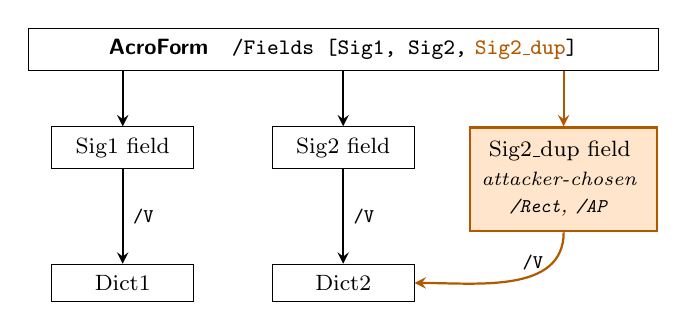
\begin{tikzpicture}[
				box/.style={draw, rectangle, align=center, inner sep=4pt, font=\footnotesize, minimum width=1.8cm},
				newbox/.style={box, fill=orange!20, draw=orange!70!black, thick},
				arr/.style={->, thick, >=stealth},
				newarr/.style={->, thick, >=stealth, draw=orange!70!black},
			]
			% AcroForm
			\node[box, minimum width=8cm] (acro) {%
			\textbf{\sffamily AcroForm}\quad\texttt{/Fields [Sig1, Sig2,} \textcolor{orange!70!black}{\texttt{Sig2\_dup}}\texttt{]}%
			};

			% Fields
			\node[box, below=0.7cm of acro, xshift=-2.8cm] (s1) {Sig1 field};
			\node[box, below=0.7cm of acro]                (s2) {Sig2 field};
			\node[newbox, below=0.7cm of acro, xshift=2.8cm] (sdup) {%
				\begin{tabular}{@{}c@{}}
					Sig2\_dup field                    \\[1pt]
					\emph{\scriptsize attacker-chosen} \\
					\emph{\scriptsize \texttt{/Rect}, \texttt{/AP}}
				\end{tabular}
			};

			% Dicts
			\node[box, below=1.2cm of s1] (d1) {Dict1};
			\node[box, below=1.2cm of s2] (d2) {Dict2};

			% AcroForm -> fields
			\draw[arr]    (acro.south -| s1.north)   -- (s1.north);
			\draw[arr]    (acro.south -| s2.north)   -- (s2.north);
			\draw[newarr] (acro.south -| sdup.north) -- (sdup.north);

			% Fields -> dicts
			\draw[arr] (s1) -- node[right, font=\scriptsize] {\texttt{/V}} (d1);
			\draw[arr] (s2) -- node[right, font=\scriptsize] {\texttt{/V}} (d2);
			\draw[newarr] (sdup.south) to[out=-90, in=0]
			node[above right, font=\scriptsize] {\texttt{/V}} (d2.east);
		\end{tikzpicture}\\[3pt]
		{\footnotesize (b) Abstract structural change (new field and edges in orange). A new signature field \texttt{Sig2\_dup} is appended to the AcroForm's \texttt{/Fields} array; its \texttt{/V} entry points at \texttt{Dict2}, the same signature dictionary already referenced by \texttt{Sig2}, while its \texttt{/Rect} and \texttt{/AP} are chosen by the attacker. The field is registered on an attacker-chosen page via that page's \texttt{/Annots} array.}
	\end{minipage}
	\caption{SFDA applied to a document containing two valid signatures: (a) visual example of the attack; (b) abstract structural view of the duplicated signature field.\label{fig:sfda-example}}
\end{figure}

\subsection{Root Cause}

Both passages quoted above overlook how their rules interact with \texttt{incremental updates}. Filling a signature field and referencing a signature dictionary are each defined as a single event, at the moment a form is completed within one static revision. The specification never asks what should happen if a signature field is filled again in a later revision, after it was already filled once, nor what should happen if a second field is created in a later revision and pointed at a signature dictionary already established in an earlier one. ASA exploits the first gap and SFDA the second.

\subsection{Limitations}

ASA can only modify an existing signature field, and is therefore constrained by the page it is presented. Documents that place signature fields on a dedicated signature page consequently offer a smaller attack surface than documents where signature fields appear alongside important content. SFDA is not bound by this same placement constraint, but it introduces a duplicated signature field that remains visible within UI-layer~2, so an attentive user could detect it.

Both attacks also depend on how tolerant a verifier is of post-signing modification, and on the permission configuration chosen when the document was signed. Some verifiers reject both attacks outright by treating any post-signing change, including benign ones, as invalidating, while others only reject them once a protection mechanism is explicitly configured, or once the modified or duplicated field is moved to a different page (Section~\ref{sec:evaluation}).

Because both attacks abuse visual components of interactive fields, their rendering can vary across readers, which may highlight the field, make it clickable, or block text selection. Such artifacts can expose the attack to an attentive user, but prior work shows users still perform security-sensitive actions when inconsistencies are small~\cite{phishing-password-managers}; in our setting they may be dismissed as reader quirks, especially when all signatures are reported valid. Prior PDF-signature attacks left similar subtle inconsistencies~\cite{pdf-certification-attack}.



\section{Methodology} \label{sec:methodology}

We evaluate 17 verifiers spanning three categories against the Appearance Substitution Attack (ASA) and the Signature Field Duplication Attack (SFDA), classifying each outcome under the criteria of Section~\ref{sec:winning-conditions}. The four GUI verifiers are Adobe Acrobat~\cite{adobereader}, Foxit PDF Reader~\cite{foxitreader}, Master PDF Editor~\cite{masterpdfeditor}, and Microsoft Edge~\cite{microsoftedge}. The two library verifiers are pyHanko~\cite{pyhanko} and the European Commission's Digital Signature Services~\cite{eudss}. The eleven web verifiers are the DSS Demonstration WebApp~\cite{dssdemo}, the ITI signature validator~\cite{itivalidador}, Certisign~\cite{certisign}, DigitalSign~\cite{digitalsign}, the Finnish DVV validator~\cite{dvv}, BRY Verifica~\cite{bry}, ZapSign~\cite{zapsign}, Clicksign~\cite{clicksign}, ON-RCPN~\cite{onrcpn}, RNP~\cite{rnp}, and CenturySign~\cite{centurysign}.

We use two testing strategies. For library verifiers and GUI desktop verifiers, where the trust anchors can be freely chosen, an automated tester (Section~\ref{sec:automated-tester}) evaluates every verifier against many possible attack configurations. For GUI web verifiers, whose trusted certificate lists are fixed by the creator and signatures with arbitrary parameters cannot be easily created, we perform a manual evaluation in which a single document carrying a signature accepted by the verifier is subjected to each attack. In both cases, we record the UI-Layer~1 and UI-Layer~2 outcomes for GUI verifiers, or the API-Layer outcome for library verifiers, and label each as \emph{vulnerable}, \emph{partially vulnerable}, or \emph{secure}.

Large Language Models such as Claude and Gemini were used for aiding on the implementation of the automated testing tool, the detection tool and for the production of figures within this paper.


\subsection{Automated Tester} \label{sec:automated-tester}

The automated tester is composed of two execution flows: test-case generation and test execution. Test-case generation enumerates configurations of the trusted signature and, for each configuration, produces one PDF carrying the corresponding ASA attack and one PDF carrying the corresponding SFDA attack. Each generated file is persisted, together with its expected verdict, in a local database for use by later runs.
%
%To generate test cases, we enumerate all combinations of the following parameters, except for the invalid case in which the signature is a certification signature and the MDP level is not defined.
%
%\begin{itemize}
%	\item $is\_certification\_signature \in \{true, false\}$: defines whether the trusted signature is a \texttt{certification} signature or an \texttt{approval} signature.
%	\item $mdp\_level \in \{null, 1, 2, 3\}$: defines the permission level. If it is \emph{null} and the signature is an approval signature, no protection mechanism is included. If it is not \emph{null}, certification signatures use \texttt{/DocMDP}, while approval signatures use \texttt{SigFieldLock}, both configured with the selected permission level.
%	\item $is\_signature\_field\_protected \in \{true, false\}$: defines whether the trusted signature field is protected by \texttt{FieldMDP}.
%	\item $is\_stamp\_enabled \in \{true, false\}$: defines whether the trusted signature has a preexisting visual component.
%	\item $change\_page \in \{true, false\}$: defines whether the modified or duplicated signature field should be placed on the same page as the original field.
%\end{itemize}

For library verifiers, each test case is submitted through the relevant verification function and the returned verdict and modification warnings are stored directly, populating the API-Layer from the layered model. For GUI desktop verifiers, the tester follows the screenshot-based approach of previous works~\cite{pdf-certification-attack}: it opens the document in the verifier, captures one screenshot per UI layer being evaluated, and classifies each by template matching against a small reference-image set per verifier and layer, one set per outcome class (\emph{valid}, \emph{warn}, \emph{invalid}). The \emph{warn} class captures the partial-vulnerability case of Section~\ref{sec:winning-conditions}, in which the verifier accepts the signature but raises a warning that the document was modified after signing.

The self-issued certificate used to produce trusted signatures for the automated tester uses a 2048-bit RSA key and a SHA-256 signature. For web verifiers, whose accepted certificate chains cannot be extended by an outside party, we instead used arbitrary documents already carrying a signature issued by a CA the verifier already trusts. The template-matching classifier described above accepts a match once the normalized cross-correlation coefficient between a screenshot and a reference image reaches at least 0.95. % TODO: say it can fail

\section{Evaluation} \label{sec:evaluation}

\begin{table}[htb]
	\centering
	\caption{Per-verifier results of how each verifier handles ASA and SFDA. \CIRCLE~means a verifier is fully \emph{vulnerable} and does not warn that modifications were made despite the signature being valid. \LEFTcircle~means a verifier is \emph{partially vulnerable} and warns that a modification occurred. \Circle~means a verifier is \emph{secure} and correctly invalidates the signature. Empty cells are layers that do not apply to the verifier's class or versions not exposed by the verifier.}
	\footnotesize
	\begin{tabular}{@{}lllccc@{}}
		\hline
		\textbf{Application}                                        & \textbf{Version} & \textbf{Category} & \textbf{UI-Layer 1}            & \textbf{UI-Layer 2}            & \textbf{API-Layer}         \\
		                                                            &                  &                   & ASA\hspace{4pt}SFDA            & ASA\hspace{4pt}SFDA            & ASA\hspace{4pt}SFDA        \\
		\hline
		Adobe Acrobat                                               & 26.1.21563.0     & desktop           & \LEFTcircle\hspace{4pt}\CIRCLE & \LEFTcircle\hspace{4pt}\CIRCLE &                            \\
		Foxit PDF Reader                                            & 2026.1.1.36485   & desktop           & \CIRCLE\hspace{4pt}\CIRCLE     & \LEFTcircle\hspace{4pt}\Circle &                            \\
		Master PDF Editor                                           & 5.9.9.8          & desktop           & \CIRCLE\hspace{4pt}\CIRCLE     & \CIRCLE\hspace{4pt}\CIRCLE     &                            \\
		Microsoft Edge                                              & 148.0.3967.83    & desktop           & \CIRCLE\hspace{4pt}\CIRCLE     & \CIRCLE\hspace{4pt}\CIRCLE     &                            \\
		pyHanko                                                     & 0.31.0           & library           &                                &                                & \Circle\hspace{4pt}\CIRCLE \\
		DSS                                                         & 6.4              & library           &                                &                                & \CIRCLE\hspace{4pt}\Circle \\
		DSS Demo WebApp                                             & 6.4              & web               & \LEFTcircle\hspace{4pt}\Circle & \LEFTcircle\hspace{4pt}\Circle &                            \\
		ITI Validador                                               & 6aec769          & web               & \CIRCLE\hspace{4pt}\Circle     & \CIRCLE\hspace{4pt}\Circle     &                            \\
		Certisign                                                   &                  & web               & \CIRCLE\hspace{4pt}\CIRCLE     & \CIRCLE\hspace{4pt}\CIRCLE     &                            \\
		DigitalSign                                                 &                  & web               & \LEFTcircle\hspace{4pt}\Circle & \LEFTcircle\hspace{4pt}\Circle &                            \\
		DVV                                                         &                  & web               & \LEFTcircle\hspace{4pt}\Circle & \LEFTcircle\hspace{4pt}\Circle &                            \\
		BRY Verifica                                                &                  & web               & \CIRCLE\hspace{4pt}\LEFTcircle & \CIRCLE\hspace{4pt}\LEFTcircle &                            \\
		ZapSign                                                     &                  & web               & \Circle\hspace{4pt}\Circle     & \Circle\hspace{4pt}\Circle     &                            \\
		ON-RCPN                                                     &                  & web               & \Circle\hspace{4pt}\Circle     & \Circle\hspace{4pt}\Circle     &                            \\
		Clicksign                                                   &                  & web               & \CIRCLE\hspace{4pt}\CIRCLE     & \CIRCLE\hspace{4pt}\CIRCLE     &                            \\
		RNP                                                         &                  & web               & \CIRCLE\hspace{4pt}\Circle     & \CIRCLE\hspace{4pt}\Circle     &                            \\
		CenturySign                                                 &                  & web               & \Circle\hspace{4pt}\Circle     & \Circle\hspace{4pt}\Circle     &                            \\
		\hline
		\multicolumn{3}{@{}l}{\textbf{ASA, vulnerable or partial}}  & 12/15            & 12/15             & 1/2                                                                                          \\
		\multicolumn{3}{@{}l}{\textbf{SFDA, vulnerable or partial}} & 7/15             & 6/15              & 1/2                                                                                          \\
		\hline
	\end{tabular}
	\label{tab:results}
\end{table}

All results in Table~\ref{tab:results} are tied to the specific software versions listed and reflect the state of each verifier at the time of testing. Vendors may patch the underlying issue in later releases, particularly following the disclosure notifications described in Section~\ref{sec:ethics}. We therefore treat these results as a snapshot rather than a permanent characterization of each product.

Our evaluation covers 11 web-based, 4 desktop, and 2 library verifiers. Desktop and library verifiers, which support automation, were each evaluated against 112 crafted PDF documents; web verifiers were evaluated manually with a single document carrying a signature trusted by each verifier. Desktop tests ran on Windows 11, web tests on Windows 11 with Microsoft Edge, and library tests on NixOS 26. Signatures for the automated tests were produced by a custom pyHanko script using a self-issued certificate.

As Table~\ref{tab:results} shows, the large majority of verifiers are vulnerable to ASA at \textbf{UI-Layer~1} or the \textbf{API-Layer}, the layers users rely on to judge whether a signature is valid. With the sole exception of Foxit, every GUI verifier vulnerable to ASA at \textbf{UI-Layer~1} is also vulnerable at \textbf{UI-Layer~2}, so the detail panel rarely catches the attack even when the user opens it. By the criteria of Section~\ref{sec:winning-conditions}, this yields 8 \emph{successful} attacks and 5 \emph{partially successful} ones.

SFDA reaches slightly fewer verifiers than ASA, with exactly half of the GUI and library verifiers reporting the signature as valid in some form at \textbf{UI-Layer~1} or the \textbf{API-Layer}. As with ASA, Foxit is the only GUI verifier whose verdict downgrades between UI layers, going from fully vulnerable at \textbf{UI-Layer~1} to \emph{secure} at \textbf{UI-Layer~2}. Overall, SFDA yields 6 \emph{successful} attacks and 2 \emph{partially successful} ones.

Foxit's downgrade between UI layers reflects how it renders \textbf{UI-Layer~1}. Inspecting the automated test outputs, we observed that even when the underlying checks detect post-signing modifications, the top bar shows only a green ``certified document'' icon and no further detail. The warnings driving the partial \textbf{UI-Layer~2} verdict for ASA, and the \emph{secure} veredict for SFDA, only appear once the user opens the per-signature detail panel.

The page-change variants of the two attacks behave asymmetrically. Every verifier vulnerable to SFDA at \textbf{UI-Layer~1} remains vulnerable when the duplicated signature field is placed on a different page. This is arguably the stronger variant, since it lets the attacker stage the forged appearance over arbitrary content on any page. The same does not hold for ASA, where DSS, ITI, BRY, and DigitalSign all reject the attack once the modified signature field is relocated to a different page.

The pyHanko library is vulnerable to SFDA only when neither \texttt{DocMDP} nor \texttt{SigFieldLock} is present, and rejects both attacks otherwise. DSS exhibits a similar behavior for ASA, accepting the attack only when the modified signature field originally defined an invisible signature. Other verifiers built on DSS, such as the DSS Demo WebApp and DVV, are plausibly vulnerable in the same configuration, but we could not confirm it, as no documents carrying an invisible signature trusted by these verifiers were available. ZapSign rejects both attacks, but does so by treating any post-signing modification as invalidating, including benign ones. In our tests, even appending a comment or a new revision to a signed document was enough to invalidate the signature.



\section{Countermeasures} \label{sec:countermeasures}

We propose countermeasures for both attacks at three levels: the specification, individual verifiers, and external detection tooling.
%
As outlined in Section~\ref{sec:attack-definitions}, both attacks exploit ambiguities in the PDF specification that allow a document's visual content to be modified without invalidating the signature.% ASA leverages the absence of a precise definition of what \emph{filling} a signature field entails, which lets verifiers treat post-signing changes to \texttt{/AP} and \texttt{/Rect} as non-invalidating. SFDA leverages the absence of any prescribed behavior when multiple signature fields reference the same signature dictionary, which lets an attacker introduce a duplicate field that the verifier renders as a valid signature.

The specification can close both gaps. To prevent ASA, ISO~32000-2 should require that any modification to the \texttt{/AP} or \texttt{/Rect} of a filled signature field invalidates the protecting signature, regardless of the prevailing \texttt{DocMDP} or \texttt{SigFieldLock} permission level. To prevent SFDA, it should require that no two signature fields reference the same signature dictionary, or, as a weaker but still sufficient alternative, that all fields referencing a given signature dictionary already exist when the dictionary is created.

Individual verifier implementations can adopt both of the above rules without waiting for the specification to change. This precedent already exists since many of the attacks reported in prior work~\cite{pdf-certification-attack,shadow-attacks,processing-dangerous-paths,one-trillion-dollar-refund,practical-decryption-exfiltration} were addressed by individual verifier vendors rather than by amendments to ISO~32000. Verifier-level mitigation, however, does not scale; every new verifier implementation can reintroduce the same class of vulnerability present in old versions of more mature verifiers.

We provide a Python tool that takes a PDF as input and produces a textual report indicating whether either attack is present. When an attack is detected, the report identifies the affected signature fields and the offending PDF objects. ASA is detected by comparing each signature field as it appears in the revision that signed it against its appearance in the latest revision; if \texttt{/AP} or \texttt{/Rect} differ, the document is flagged. SFDA is detected by scanning the latest revision for pairs of signature fields that reference the same signature dictionary and verifying, for each pair, whether at least one of the fields was introduced in an incremental update later than the dictionary it references.


\section{Related Works} \label{sec:related-works}

One Trillion Dollar Refund~\cite{one-trillion-dollar-refund} presented three attacks against approval-signature verifiers. The Universal Signature Forgery (USF) changes the signature dictionary so the verifier cannot find what it needs but still reports the signature as valid. The Incremental Saving Attack (ISA) appends a broken incremental update that adds visual modification. The Signature Wrapping Attack (SWA) moves the signed bytes elsewhere and puts new content in place.

Subsequent work introduced shadow attacks~\cite{shadow-attacks}, building on top of~\cite{one-trillion-dollar-refund}, which use spec-compliant incremental updates instead of broken ones. Their attack plants hidden content in the document before it is signed and reveals it afterwards through normal incremental updates.

In contrast, later work examined certification signatures and identified two attacks~\cite{pdf-certification-attack}. The Evil Annotation Attack (EAA) adds annotations that hide or replace certified content. The Sneaky Signature Attack (SSA) adds a new signature whose appearance covers attacker-controlled content. Both attacks abuse changes that \texttt{DocMDP} allows. SSA also requires the attacker to get a fresh certificate trusted by the verifier, since the new signature has to be considered valid.

Unlike USF, ISA, and SWA, ASA uses solely incremental updates fully within the spec. Unlike the shadow attacks, ASA needs no access to the document before signing and can be applied to any already-signed PDF. The closest match is EAA, which also covers the page with attacker-chosen content, but through a new annotation governed by \texttt{DocMDP}/\texttt{SigFieldLock} annotation permissions, ASA instead changes the signature field's own \texttt{/AP} and \texttt{/Rect}, which affected verifiers treat as part of filling the field, letting it work at lower permission levels than EAA.

SFDA also works only on already-signed PDFs and follows the spec. The closest match is SSA, since both add a new signature field the verifier shows as valid, but SSA brings its own signature dictionary, forcing the attacker to obtain a trusted certificate, while SFDA points the new field at a signature dictionary already present in the document. This widens the threat to settings where a trusted certificate is hard to get, such as documents signed under closed PKIs, and the duplicated field inherits the original signer's name and certificate chain, making the forgery harder to dismiss than SSA's unfamiliar identity.

Table~\ref{tab:comparison-matrix} summarizes the attacks discussed above along the dimensions that separate them.

\begin{table}[htb]
	\centering
	\footnotesize
	\resizebox{\linewidth}{!}{%
	\begin{tabular}{@{}l c c c c l@{}}
		\hline
		\textbf{Attack}                       & \textbf{Spec-comp.?} & \textbf{Pre-sign?} & \textbf{Own cert.?} & \textbf{MDP~2?} & \textbf{Targets}                          \\
		\hline
		USF~\cite{one-trillion-dollar-refund} & No                   & No                 & No                  & No              & Signature dictionary                      \\
		ISA~\cite{one-trillion-dollar-refund} & No                   & No                 & No                  & No              & Xref table / trailer                      \\
		SWA~\cite{one-trillion-dollar-refund} & No                   & No                 & No                  & No              & Signed byte range                         \\
		Shadow~\cite{shadow-attacks}          & Yes                  & Yes                & No                  & No              & Hidden content                            \\
		EAA~\cite{pdf-certification-attack}   & Yes                  & No                 & No                  & No              & Annotations                               \\
		SSA~\cite{pdf-certification-attack}   & Yes                  & No                 & Yes                 & Yes             & New signature field                       \\
		\textbf{ASA (ours)}                   & Yes                  & No                 & No                  & Yes             & Sig. field (\texttt{/AP}, \texttt{/Rect}) \\
		\textbf{SFDA (ours)}                  & Yes                  & No                 & No                  & Yes             & Sig. field duplication                    \\
		\hline
	\end{tabular}%
	}
	\caption{Comparison of PDF signature-forgery attacks.}
	\label{tab:comparison-matrix}
\end{table}


\section{Ethical Considerations and Responsible Disclosure} \label{sec:ethics}

This paper demonstrates practical attacks against 17 signature verifiers, several of which are commercial products in wide use. We follow a coordinated disclosure process to notify affected vendors before these findings are made public.

We have notified the vendor or maintainer of every verifier found vulnerable or partially vulnerable to ASA or SFDA under the criteria of Section~\ref{sec:winning-conditions}, and are working with each toward a fix. We follow a 30-day disclosure window per vendor, counted from the date of notification. Because not every vendor has shipped a fix as of this submission, we cannot yet publish a complete table of dates; we will publish the affected verifiers and their fixed versions at \url{TODO} once every vendor has fixed the issue or reached the end of its window, or otherwise in an updated version of this paper before final publication. % TODO: fill in artifact/tracking URL before camera-ready

We release the detection tool of Section~\ref{sec:countermeasures} in full, and a simplified version of the test-case generation framework of Section~\ref{sec:methodology} that omits the code assembling a concrete attack chain, as part of the SBSeg artifact submission. We withhold the full generation framework and the malicious PDFs produced during our evaluation until the targeted verifier has been fixed or its disclosure window has closed.


\section{Conclusion} \label{sec:conclusion}

PDF signatures provide a standardized and consistent way for someone to approve the state of a document at a specific instant of time. However, visual modifications can be made by incrementally updating the document in a way that keeps the signature itself valid and triggers no modification warning. In this paper, we introduced two novel attacks that abuse flaws in the specification, the Appearance Substitution Attack (ASA) and the Signature Field Duplication Attack (SFDA). Although neither modifies the page directly, both abuse the appearance mechanism of interactive forms to overlay visual changes on top of the page, and even when detectable the result is subtle enough that most users would not hesitate to trust the signature, since affected verifiers still report it as valid and do not flag the modifications. We then evaluated these attacks against many verifiers and found that most were vulnerable in one way or another.

Although we proposed countermeasures to mitigate the damage such attacks can cause, both this work and previous attacks can be seen as proof that the large complexity of the PDF specification, coupled with the decentralized ecosystem where each verifier implements its own algorithm and interprets the ISO in its own way, creates fertile ground for attacks of this kind. In fact, one could argue that incremental updates, which greatly complicate signature validation, are themselves a dangerous functionality, given that both the attacks introduced here and more than half of those in Section~\ref{sec:related-works} abuse incremental updates in one way or another. As future work, it would be valuable to define a standardized verification algorithm on which all verifiers could base their implementations.

\section*{Acknowledgements}

This research was partially financed by ON-RCPN.



\bibliographystyle{sbc}
\bibliography{sbc-template}

\end{document}


